\documentclass[12pt]{article}

% Packages:
\usepackage{graphicx}
\usepackage[portuguese]{babel}
\usepackage[utf8]{inputenc}
\usepackage{setspace}
\usepackage{listings}
\usepackage{hyperref}
\usepackage{tocloft}
\usepackage{fancyhdr}
\usepackage{placeins}
\usepackage{subcaption}
\usepackage{subfiles}
\usepackage{outlines}
\usepackage{indentfirst}
\usepackage{amsmath}
\usepackage{enumerate}
\usepackage{subfiles}
\usepackage{color, colortbl, xcolor}
\usepackage{multicol}
%---

% Options:
\setstretch{1} % Espaçamento entre linhas
\usepackage[top=3cm, bottom=2cm, left=1.5cm, right=1.5cm]{geometry}
\PassOptionsToPackage{hyphens}{url}
\title{}
\date{}

% Code customization:
% Default fixed font does not support bold face
\DeclareFixedFont{\ttb}{T1}{txtt}{bx}{n}{10} % for bold
\DeclareFixedFont{\ttm}{T1}{txtt}{m}{n}{10}  % for normal

\lstset{
	basicstyle=\footnotesize,
	columns=fullflexible,
    keywordstyle=\ttb\color{blue},
	stringstyle=\ttm\color{green},
	commentstyle=\color{gray},
	frame=None,
	breaklines=true,
	showstringspaces=false,
	postbreak=\mbox{\textcolor{red}{$\hookrightarrow$}\space},
}

\lstdefinestyle{R} {
	language=R,
	keywordstyle=\ttb\color{blue},      % keyword style
	stringstyle=\ttm\color{purple},     % string literal style
	deletekeywords ={seq,end},
	frame=single,
	numbers=left
}

%---
% Document:
\begin{document}
	% Cabeçalho:
\begin{figure}
		\begin{minipage}{.3\linewidth}
			\centering
			
\includegraphics[width=.6\linewidth]{imgs/ufpa.jpg}
		\end{minipage}
		\begin{minipage}{.70\linewidth}
			\flushleft
			\paragraph{}
			\textbf{ }\newline
			\textbf{UNIVERSIDADE FEDERAL DO PARÁ} \newline
			\textbf{INSTITUTO DE TECNOLOGIA} \newline
			\textbf{FACULDADE DE ENGENHARIA DA COMPUTAÇÃO E TELECOMUNICAÇÕES} \newline
			\textbf{TE05205 - Top. Especiais em Engenharia de Computação II} \newline
            \textbf{Prof. Dr. Roberto Celio Limão de Oliveira} \newline
            \textbf{Aluna: Camila Novaes Silva (201606840055)}
		\end{minipage}
\end{figure}
\FloatBarrier
\begin{center}
    {\Large \textbf{Algoritmos Genéticos}}
\end{center}
%%%%%%%%%%%%%

\section{Introdução}
Algoritmos genéticos (AG) são uma classe particular de algoritmo evolutivo que usam técnicas
inspiradas pela biologia evolutiva. Esses algoritmos são muito eficientes para busca de
soluções ótimas, ou aproximadamente ótima em uma grande variedade de problemas.

\section{Características e Componentes}
Nos algoritimo genéticos, o indivíduo, ou cromossomo, é a estrutura principal que abrigará
uma possível solução para o problema proposto e o conjunto desses elementos formam uma
população. Em geral, um indivíduo é representado por uma cadeia de genes de tamanho fixo,
que são representadas através de vetores. Cada posição do vetor, denominada lócus, é
análoga aos genes de um cromossomo. Assim, o valor de uma posição do vetor ou da cadeia
representa um alelo do cromossomo.

Os alelos estão contidos dentro de um conjunto de possíveis valores que poderão ser assumidos.
Esse conjunto é denominado de alfabeto. O alfabeto está intrinsecamente relacionado ao problema
a ser resolvido, tendo em vista que ele define os possíveis valores que irão preencher os
cromossomos ou indivíduos.

O algoritimo genético requer uma função que defina um grau de adaptação ao meio, o
\textit{fitness}, aplicado a cada um de seus indivíduos. O \textit{fitness} mede a capacidade
de cada cromossomo de resolver o problema avaliado. A "qualidade" de um cromossomo é estimada
com base em seu \textit{fitness}. Dessa forma, indivíduo com melhor \textit{fitness} terão maior
probabilidade de sobreviver e participar de operações de cruzamento, dando origem a novos
indivíduo.

Assim, um algoritimo genético simples consiste em: (1) inicializar uma população de
possíveis soluções, (2) cada indivíduo da população é avaliado por uma função de avaliação
(fitness), (3) os pais são selecionados para a reprodução, (4) realiza-se o cruzamento e a
mutação. Assim, os passos de 2 a 4 são repetidos até que determinado critério seja atingido,
como obtenção de uma solução satisfatória para o problema ou o esgotamento do tempo disponível
para processamento.

\section{Seleção}
A operação de seleção determinada quais cromossomos participarão da produção de uma nova geração
através de operações de cruzamento (reprodução). Em geral, os membros são selecionados com base
em critérios proporcionais ao seu fitness. Existem diversos métodos de seleção, dentre eles:

\begin{enumerate}[\textbf{(i)}]
	\item \textbf{Roleta Simples Proporcional}: Este método representa a populaçao em forma de
		  uma roleta, em que cada fatia representa um indivíduo e tem tamanho proporcional ao
		  seu \textit{fitness}. Assim, cada vez que a roleta é girada, um indivíduo é selecionado
		  para a reprodução.

	\item \textbf{Roleta Simples Ranking}: Assim como a Roleta simples Proporcional, tende a
		  favorecer os indivíduos com maior \textit{fitness}, porém, na seleção por ranking, a
		  informação do \textit{fitness} é descartada e apenas o desempenho de cada indivíduo em
		  relação aos demais é levada em consideração.

	\item \textbf{Torneio}: A seleção por torneio consiste na definição de um grupo aleatório de
		  indivíduo da população. Dos indivíduos escolhidos aleatoriamente, o melhor será
		  selecionado. O processo é repetido até que seja alcançado o número de indivíduos que
		  devem se reproduzir.

\end{enumerate}

\section{Operadores Genéticos}
A reprodução dos indivíduos existentes em uma população se dá através de operações capazes de
recombinar e modificar os genes de seus cromossomos. A principal função dos operadores genéticos
é dar origem a novos indivíduos que preservam características de seus "pais", assim como ocorre
na evolução natural.

Alguns dos principais operadores genéticos, são:
\begin{enumerate}[\textbf{(i)}]
	\item \textbf{Cruzamento}: O cruzamento, também chamado de recombinação, é a operação que
		  gera dois novos indivíduos, os filhos, a partir da combinação do material genético
		  de dois outros indivíduos, os pais.
		  Existem diversas formas de cruzamento, dentre elas:
		  \begin{itemize}
			\item \textbf{Um ponto de corte}: Os dois cromossomos "pais" devem sofrer um corte
			em uma região aleatória e a partir deste ponto as informações genéticas dos pais
			serão trocadas e assim, os dois cromossomos "filhos" serão gerados.
			\item \textbf{Vários pontos de corte}: Duas ou mais posições aleatórias são
			definidas para corte dos cromossomos pais.
			\item \textbf{Máscara Binária}: Defini-se um vetor binário, chamado de máscara
			binária, do mesmo tamanho do cromossomo utilizado, onde para cada posição da
			máscara, se o valor for 1, o primeiro filho herda o gene do primeiro pai e o
			segundo filho herda o gene do segundo pai; se o valor for 0, o inverso acontece.
		  \end{itemize}
	\item \textbf{Mutação}: A mutação é um operador de age sobre um único indivíduo por vez.
		  Esse operador modifica o valor de um gene aleatório de um indivíduo. Ao modificar
		  o valor do gene, a mutação pode introduzir em um indivíduo novos genes, o que
		  ajuda a aumentar a diversidade populacional.

\end{enumerate}

\section{Exemplo de AG: Container de frutas}
Para exemplificar a utilização de algoritimos genéticos para um problema de ótimização, foi
feita a implementação de um algoritimo para determinar o número de frutas de cada tipo que um
container pode carregar de forma a alcançar o maior valor de carregamento, sem ultrapassar o
peso máximo de 500 e respeitando o mínimo de frutas de 4 unidades.

\begin{table}[ht]
	\centering
	\begin{tabular}{|c|c|c|}
		\hline
		\rowcolor{gray}
		Fruta & Peso & Valor \\ \hline
		 Limão & 2 & 3 \\ \hline
		 Laranja & 4 & 6 \\ \hline
		 Mamão & 5 & 10 \\ \hline
		 Abacaxi & 8 & 18 \\ \hline
		 Melancia & 12 & 26 \\ \hline
	\end{tabular}
	\caption{Relação de frutas, peso e valor\label{tb:container-de-fruta}}
\end{table}

Dessa forma, utilizando as informações da tabela~\ref{tb:container-de-fruta} foi desenvolvido
um algoritmo com uma população de 2000 indivíduos, onde cada cromossomo é um vetor de 6 posições,
uma posição para cada fruta e 1 posição para o fitness. O torneio foi utilizado como algoritimo de
seleção, usando uma taxa de cruzamento de 50\%, e o algoritimo de ponto de corte foi utilizado
para cruzamento. Também, foi utilizado uma taxa de mutação de 3\%. Por fim, a condição de parada
utilizada foi de 30 gerações.

\begin{figure*}[htb]
	\begin{center}
	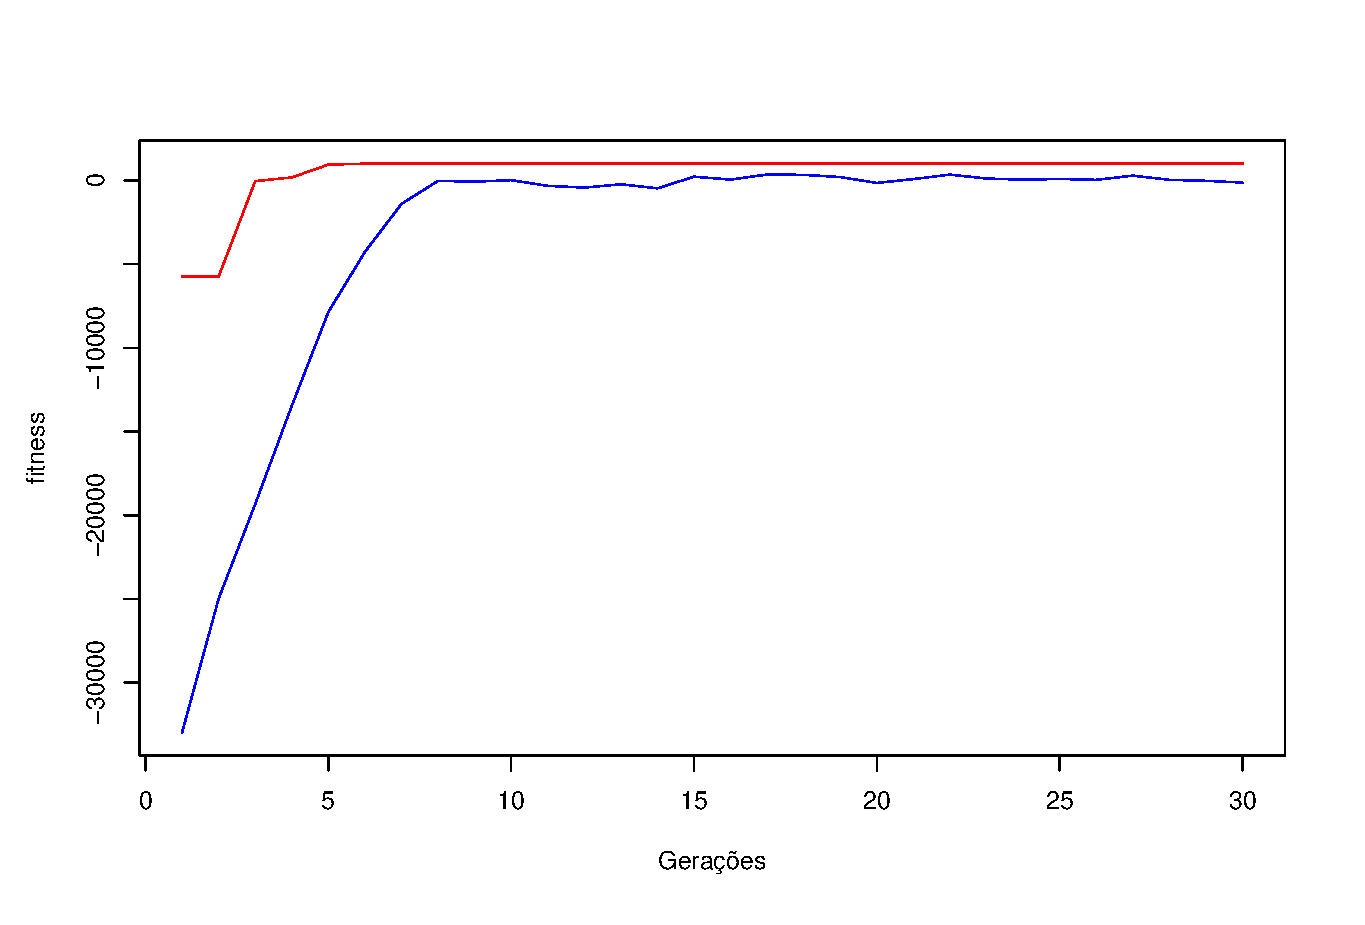
\includegraphics[width=0.6\textwidth]{./imgs/result-ag.eps}
	\caption{Resultado do AG para o problema de dimensionamento de container.\label{fig:result}}
	\end{center}
\end{figure*}

O resultado obtido pode ser visualizado na Fig.~\ref{fig:result}, onde a linha vermelha representa
a \textit{fitness} do melhor indivíduo ao longo das gerações e a linha azul, a média do \textit{fitness}
de todos os indivíduos da população. O resultado final foi: 13 limões, 4 laranjas, 10 mamãoes, 45 abacaxis
e 4 melancias.


\end{document}
